\chapter{Il Gradiente di sottosterzo}
\label{cha:cap2}
Una classica caratteristica del comportamento in curva di un veicolo, è il concetto di
sottosterzo, sovrasterzo o sterzo neutro (introdotto nella sez.\ref{Dinamica laterale}).\\
Si può esprimere questo concetto (in modo semplice) basandosi sull’interazione tra la velocità di avanzamento e la 
curvatura durante la percorrenza di una curva in condizioni stazionarie:\\
Se all’aumentare della velocità del veicolo cresce la curvatura percorsa allora 
siamo in condizione di sottosterzo.
Quando la curvatura rimane invariata all’aumentare della velocità allora siamo in
condizione di sterzo neutro.\\
Per lo studio della stabilità direzionale dei veicoli era necessario avere un indicatore intuitivo
che descrivesse le differenze tra i casi elencati;\\ 
Il gradiente di sottosterzo è un parametro chiave utilizzato per quantificare e comprendere questo
comportamento.\\
Questo concetto è stato introdotto per la prima volta da Olley nel 1946 \cite{Olley1946RoadMO}:\\
-Olley definì la "Linea di sterzo neutro" come il punto dove qualsiasi forza esterna applicata non 
produceva alcun momento d'imbardata addizionale durante una curva ed Il gradiente di sottosterzo
era la distanza longitudinale tra il centro di massa e la linea di sterzo neutro.
Sebbene non siano state ricavate espressioni matematiche questo concetto coinvolge le derivate degli
angoli di deriva dei pneumatici.\\
-A seguito dell'introduzione della sterzata cinematica (Ackermann), fù proposta un nuova formulazione definita come la differenza tra l'angolo di sterzo di riferimento e l'angolo di sterzo cinematico : $Ua_y = \delta_{REF} - \delta_A$ \cite{society1965vehicle}.\\
-Nel 1973 Pacjeka, studiò il concetto di gradiente di sottosterzo, scrivendo l'articolo \cite{doi:10.1080/00423117308968439}, nel quale presentava un metodo approssimato che permetteva di
creare un diagramma (handling diagram) utile per analizzare la stabilità in curva di un veicolo 
stradale in condizioni stazionarie.\\
Nella seconda parte dell'articolo \cite{doi:10.1080/00423117308968440} dimostrò, utilizzando il modello a singola traccia linearizzato ed esaminandone i poli, come il sottosterzo garantisca la stabilità in curva in condizioni stazionarie.\\
-Nel 1996 tramite lo standard SAE \cite{J266_201811}, si definirono le procedure per i test di controllo direzionale dei veicoli stradali, in modo da considerare le varie possibili condizioni di prova. \\
Furono apportate,inoltre, delle migliorie nella formulazione basata sulla sterzata cinematica, aggiungendo la possibilità di includere lo sterzo posteriore, in questo caso l'angolo di riferimento è dato dalla differenza tra l'angolo di sterzo anteriore e posteriore.\\
-Recentemente Guiggiani formulò delle perplessità riguardanti le definizioni del gradiente di sottosterzo esistenti, sostenendo che non fossero chiaramente definite per veicoli a 4 o più ruote.\\
In un primo momento propose un miglioramento del $K_{SAE}$ per renderlo indipendente dal passo dei veicoli.
Successivamente propose un nuovo approccio all'handling che analizzeremo in seguito.
%-------------------------------------------------------------------------------------------------------
\section{Formulazioni classiche del gradiente di sottosterzo}
Le tre formulazioni maggiormente utilizzate sono: $K_{Pacejka}$ , $K_{SAE}$ , $K_{Guiggiani}$.
\subsection{Formulazione di Pacejka}
Pacejka introdusse il concetto di gradiente di sottosterzo per veicoli a trazione anteriore (FWD), inizialmente concentrando l'attenzione su modelli lineari e successivamente estendendolo a modelli non lineari.\\
Per pneumatici lineari, le forze sono definite come $F_{yf} = C_f \alpha_f$ e $F_{yr} = C_r \alpha_r$, 
La relazione tra l'angolo di sterzo anteriore, la curvatura e la velocità può essere scritta omettendo la derivata rispetto
al tempo:\\
\begin{equation} \label{7}
\frac{1}{R} = \frac{ C_f C_r l}{C_f C_r l^2 - mu^2(C_f a - C_rb)} \delta
\end{equation}

Combinando con $\rho = \frac{r}{v_x} = \frac{1}{R}$, si ottiene:
\begin{equation} \label{8}
\delta_f = \frac{1}{R} (l - mu^2\frac{C_f a - C_r b}{l C_f C_r})
\end{equation}
il Gradiente di sottosterzo è definito con $\eta$:
\begin{equation}
    K_{Pacejka} = \eta = -\frac{mg}{l} \frac{C_fa-C_rb}{C_fC_r} = -\frac{s}{l} \frac{mgC}{C_fC_r}
\end{equation}
\begin{figure}[!h]
    \centering
    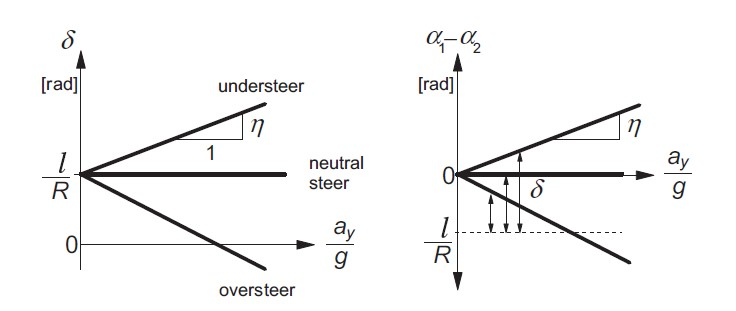
\includegraphics[scale=0.7]{Immagini/Understeer Gradient/Pacjeka understeer gradient.jpg}
    \label{fig:Pacjeka understeer gradient}
    \caption{Il gradiente di sottosterzo secondo la formulazione di Pacjeka}
\end{figure}
L'equazione \ref{7} scritta per il modello lineare può essere riscritta:\\
\begin{equation}
\delta_f = \frac{l}{R}( 1 + \eta\frac{u^2}{gl} ) = \frac{l}{R} + \eta \frac{a_y}{g}
\end{equation}
In condizioni non lineari, il gradiente di sottosterzo deriva dalla geometria (sterzata cinematica, Ackermann):\\
\begin{equation}
\frac{d\delta_f}{da_y} = \frac{d(\alpha_f - \alpha_r)}{da_y}
\end{equation}
Si può ricondurre la formulazione al $K_0$:
\begin{equation}
K_{Pacejka} = \frac{d(\alpha_f - \alpha_r)}{d(a_y/g)} = -\frac{g}{l} K_0
\end{equation}

\subsubsection{Handling Diagram}
Per migliorare la comprensione del comportamento direzionale a regime con pneumatici non lineari, si introduce un metodo
grafico per visualizzare intuitivamente la risposta del veicolo, basato sugli angoli di deriva dei pneumatici.\\
Per tracciare questo diagramma è necessario partire dalla curva che presenta nell' asse delle ascisse gli angoli di deriva
$\alpha_i$ mentre nell' asse delle ordinate la forza laterale normalizzata rispetto alla forza verticale 
$\frac{F_{yi}}{F_{zi}}$ (fig.\ref{fig:example of Handling diagram}).\\
\begin{figure}[!h]
    \centering
    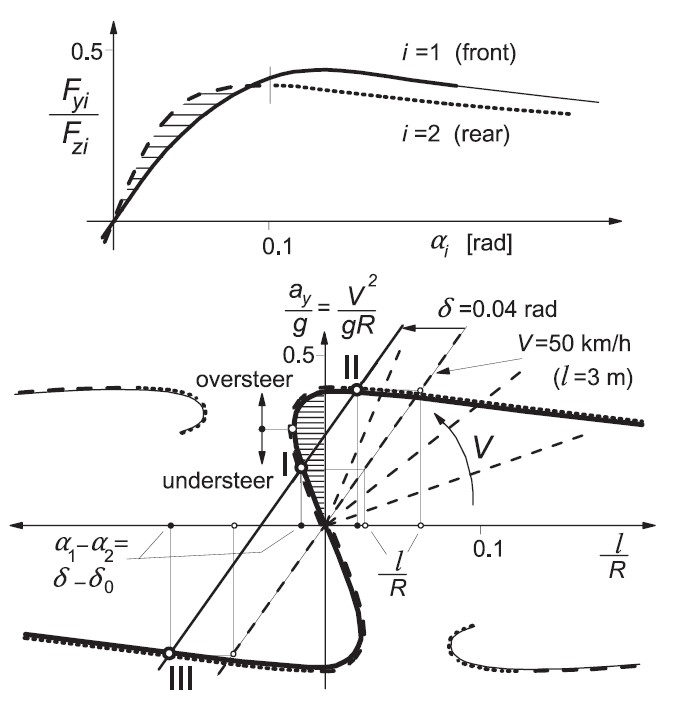
\includegraphics[scale=0.7]{Immagini/Understeer Gradient/example of handling diagram.jpg}
    \caption{handling diagram ottenuto per una velocità di 50[km/h] e $\delta$ = 0.04 [rad]}
    \label{fig:example of Handling diagram}
\end{figure}
Per ogni valore dell'ordinata si ottengono uno o più valori della differenza tra $\alpha_1 - \alpha_2$ ($\alpha_f - 
\alpha_r$); tracciando nel grafico questi valori si arriva alla definizione della funzione:
\begin{equation}
    \alpha_1 - \alpha_2 = (\delta_1 - \delta_2) - \frac{l}{R} = f(\frac{\Tilde{a_y}}{g})
\end{equation}

\begin{figure}[!h]
    \centering
    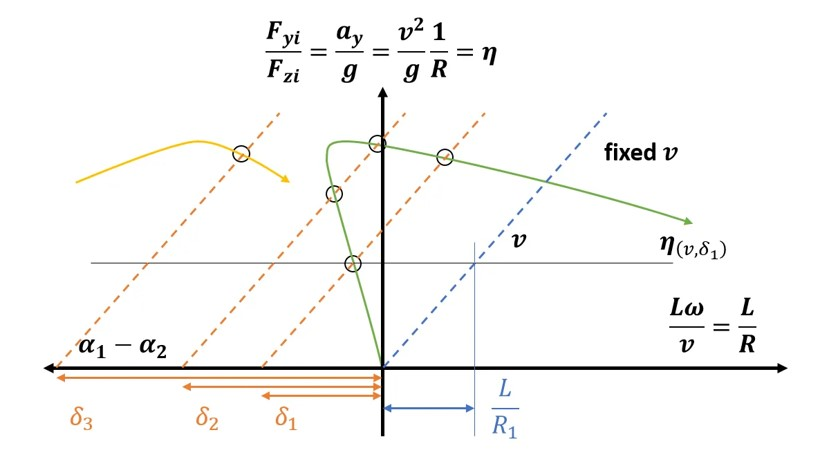
\includegraphics[scale=0.7]{Immagini/Understeer Gradient/handling diagram(2).jpg}
    \caption{}
    \label{fig:Handling Diagram2}
\end{figure}
Riferendosi alla figura \ref{fig:Handling Diagram2} si nota che "l'handlig curve" è composta da un ramo principale e da un
ramo secondario,che non dipendono dai parametri di prova ma solo dalla caratteristiche costruttive.\\
Le rette tratteggiate con coefficiente angolare $u^2/gl$ rappresentano le possibili condizioni di prova ($\delta$ e $u$):\\
Le intersezioni tra retta e curva individuano le uniche possibili condizioni di equilibrio.\\ 
\begin{figure}[!h]
    \centering
    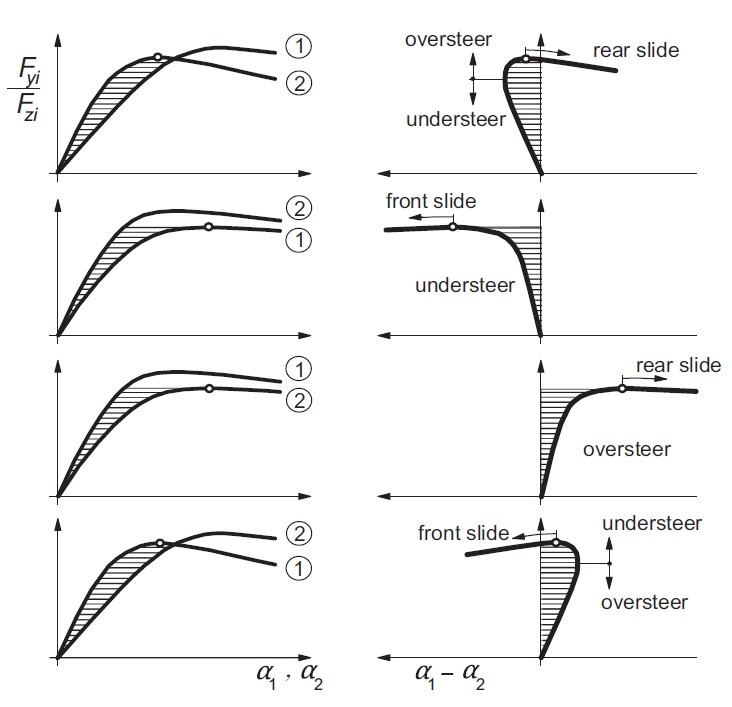
\includegraphics[scale=0.7]{Immagini/Understeer Gradient/handling Diagrams.jpg}
    \caption{Diverse tipologie di comportamento direzionale}
    \label{fig:Handling Diagrams}
\end{figure}
La figura \ref{fig:Handling Diagrams} mostra intuitivamente come le caratteristiche dei pneumatici siano responsabili del comportamento del veicolo al variare delle condizioni operative ($\Tilde{a_y}/g$) 

\subsection{Formulazione SAE}

La formulazione SAE è anch'essa basata sulla geometria della sterzata di Ackermann, considera veicoli a 4 ruote sterzanti,
definendo:\\
Angolo di sterzo di Ackermann (cinematico) come $\delta_A = \frac{L}{R}$.\\ 
Angolo di sterzo di riferimento come $\delta_{\text{ref}} = -\delta_f + \delta_r$.\\
Il gradiente di sottosterzo è infine definito come la differenza tra loro derivate:
\begin{figure}[!h]
    \centering
    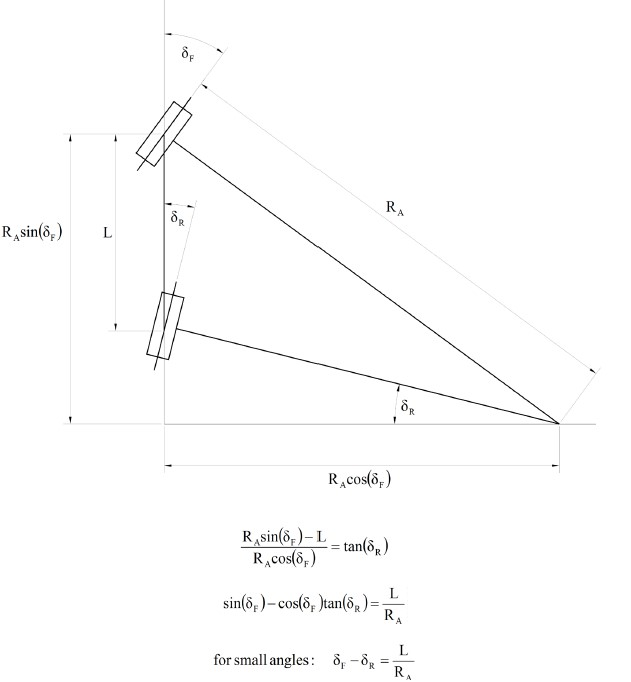
\includegraphics[scale=0.7]{Immagini/Understeer Gradient/Ackermann geometry.jpg}
    \caption{Angolo di sterzo cinematico}
    \label{fig:Delta ref}
\end{figure}
\begin{equation}
K_{SAE} = \frac{d\delta_{ref}}{da_y} - \frac{d\delta_A}{da_y} = \frac{d(-\alpha_f + \alpha_r)}{da_y}
\end{equation}
Potrebbe essere riportato al $K_0$ come segue:
\begin{equation}
K_{SAE} = l \cdot \frac{\partial \rho}{\partial a_y} = l \cdot K_0
\end{equation}



\subsection{Formulazione di Guiggiani}
Nel primo libro \cite{guiggiani2007dinamica} propose una formulazione in accordo con la definizione SAE \cite{J266_201811}:\\
\begin{equation}
    K_{\gamma} = \frac{d}{d\Tilde{a}_y} (\delta - \frac{l}{R}) = \frac{d}{d\Tilde{a}_y} (\alpha_{1p} - \alpha_{2p}) = \frac{d}{d\Tilde{a}_y} (\gamma_0 - \gamma_p)
\end{equation}
Che nel caso del modello lineare diventava:\\
\begin{equation}
    K_{\gamma} = \frac{m}{l}( \frac{\Phi_2 a_2 - \Phi_1 a_1}{\Phi_1 \Phi_2})
\end{equation}
Nella seconda edizione \cite{guiggiani2018science} criticò aspramente la definizione SAE come vedremo successivamente,
proponendo una nuova versione che migliorasse la precedente, che è funzione di due variabili:\\
\begin{equation} \label{roy 1}
    \rho_y = \rho_y(\delta_{va},\Tilde{a}_y)
\end{equation}
eccetto nel caso del modello a singola traccia con differenziale aperto,\\
allora $\rho_y = \rho_y (\Tilde{a}_y) = - df_{\rho}/d\Tilde{a}_y $ :
\begin{equation} \label{6.171}
    \rho_y = \frac{\partial \rho_p}{\partial \tilde{a}_y} = \frac{\partial}{\partial \tilde{a}_y} (\frac{1}{R}) = -\frac{K}{l}
\end{equation}
Questa è molto simile alla definizione classica del K ma con delle differenze sostanziali:\\
\'E definito per qualsiasi in quanto non è influenzato dal passo $l$ dei veicoli e neanche dallo sterzo di Ackermann.\\
Naturalmente, la derivata parziale nell'eq.\ref{6.171} richiede che l'angolo di sterzo sia mantenuto costante.
Nel caso di un test ad angolo volante fissato l'eq.\ref{6.171} può essere riscritta come:\\
\begin{equation}
    \frac{d\rho_p}{d\tilde{a}_y} = \frac{d(r_p/u_a)}{d(r_pu_a)} = \frac{d(r_p/u_a)}{du_a} (\frac{d(r_pu_a)}{du_a})^{-1} = \frac{1}{u_a^2} (\frac{\dot r_pu_a - r_p}{\dot r_pu_a + r_p}) = \rho_y
\end{equation}


\subsection{Confronto e limiti delle formulazioni classiche}

\subsubsection{Confronto}
Le tre formulazioni analizzate sono sostanzialmente equivalenti a $K_0$, condividendo la derivata 
dell'accelerazione laterale al denominatore.\\
\begin{figure}[!h]
    \centering
    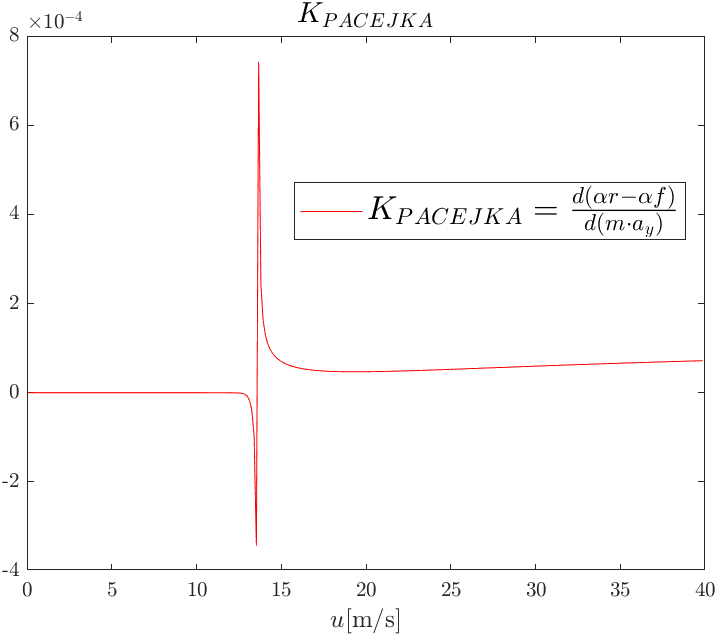
\includegraphics[scale=0.5]{Immagini/Understeer Gradient/Kpacejka.png}
    \caption{}
    \label{fig:Kpacejka}
\end{figure}
\begin{figure}[!h]
    \centering
    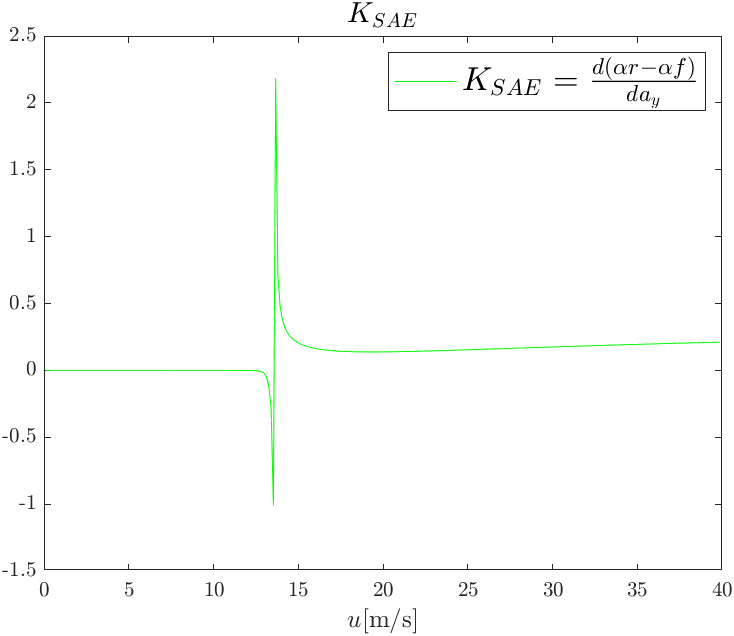
\includegraphics[scale=0.5]{Immagini/Understeer Gradient/Ksae.png}
    \caption{}
    \label{fig:Ksae}
\end{figure}
\begin{figure}[!h]
    \centering
    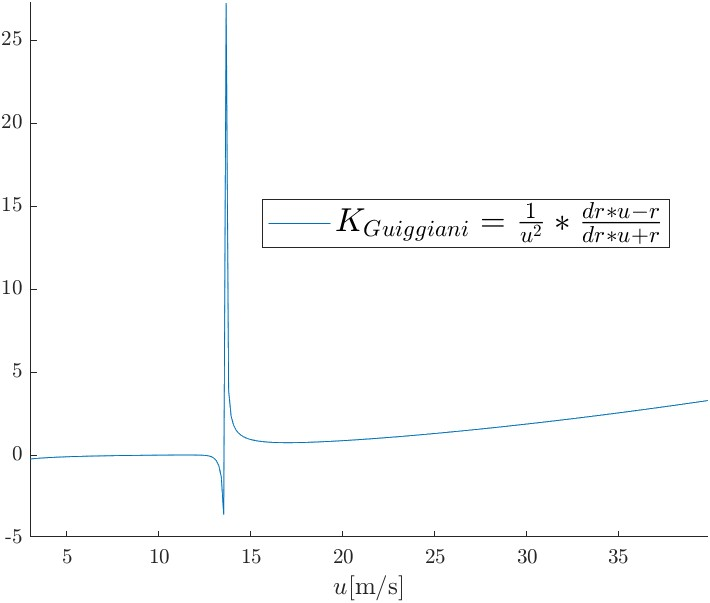
\includegraphics[scale=0.25]{Immagini/Understeer Gradient/Kguiggiani.jpg}
    \caption{}
    \label{fig:Kguiggiani}
\end{figure}

\subsubsection{Limiti}
Tutte e tre le formulazioni classiche condividono la derivata dell'accelerazione laterale al denominatore, 
questo genera una scarsa definizione nei punti di flesso.\\
Se si considerano angoli di sterzo costanti su entrambi gli assi, la derivata parziale può essere sostituita dal 
differenziale dunque $\frac{\partial \rho}{\partial a_y} \longrightarrow{} \frac{d \rho}{da_y}$. Essendo in condizioni
stazionarie, abbiamo $\rho = \frac{r}{u}$ e $a_y = r \cdot u$. Quindi, $K_0$ diventa:
\begin{equation}
K_0 = 
\frac{d \rho}{da_y} = \frac{d \left( \frac{r}{u} \right)}{d(ru)} = \frac{\frac{d(\frac{r}{u})}{du}}{\frac{dr}{du}} =
\frac{\frac{dr}{du} - \frac{r}{u}}{u^2( \frac{dr}{du} + \frac{r}{u})} =
\frac{\frac{d \rho}{du}}{u( \frac{dr}{du} + \frac{r}{u})}
\end{equation}
Il suo numeratore rappresenta esattamente il concetto di gradiente di sottosterzo, il cui segno indica la tendenza
sottosterzante, sovrasterzante o neutro.
$K_0$ descrive correttamente questa caratteristica finchè il segno del denominatore è costante. \\
Tuttavia, non è sempre costante:\\
A bassa velocità, la velocità d'imbardata ($r$) aumenta all'aumentare dell'accelerazione, $\frac{dr}{du}$ risulta
positivo, essendo il denominatore positivo. \\
Man mano che la velocità d'imbardata si avvicina al suo limite massimo correlato al limite di accelerazione laterale,
questa inizia a diminuire, $\frac{dr}{du}$ diventa negativo (fig.\ref{fig:r vs u delta=0.145}).\\ 
Di conseguenza, il denominatore potrebbe diventare zero o negativo. Questo cambiamento nel segno del denominatore
interrompe la connessione tra $K_0$ e la caratteristica di sottosterzo. Inoltre, un denominatore intorno a zero causerebbe
instabilità numerica (fig.\ref{fig:K0 delta=0.145}).\\
\begin{figure}[!h]
    \centering
    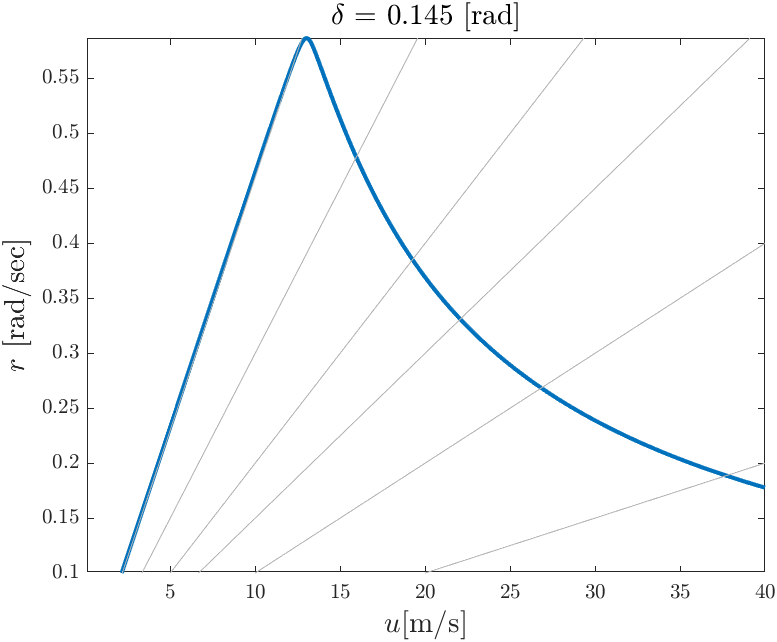
\includegraphics[scale=0.7]{Immagini/Understeer Gradient/r vs u.png}
    \caption{velocità d'imbardata e velocità}
    \label{fig:r vs u delta=0.145}
\end{figure}
\begin{figure}[!h]
    \centering
    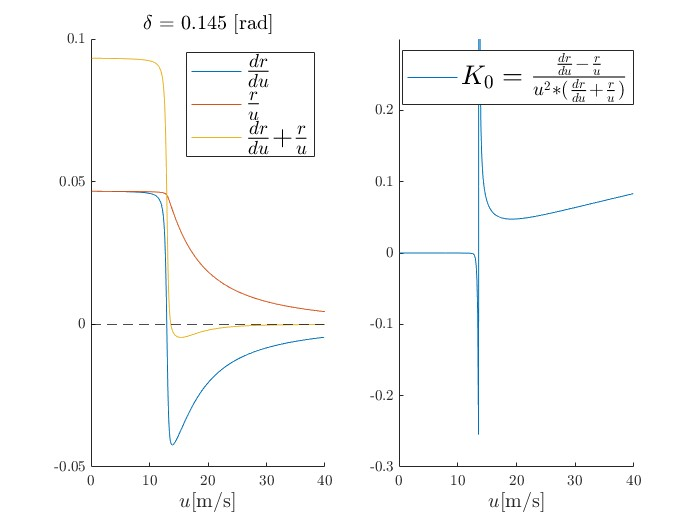
\includegraphics[scale=0.5]{Immagini/Understeer Gradient/K0.jpg}
    \caption{$K_0$}
    \label{fig:K0 delta=0.145}
\end{figure}
L'esempio mostrato nelle fig.\ref{fig:r vs u delta=0.145} e \ref{fig:K0 delta=0.145} rappresenta la velocità d'imbardata in
regime stazionario di un veicolo a trazione anteriore e pneumatici non lineari (rimandare ad appendice dove si spiega il
modello) che esegue una manovra ad angolo di sterzo fissato $\delta_f = 0.145$ e velocità crescente da 0 a 40 [m/s].\\
In particolare la fig.\ref{fig:r vs u delta=0.145} rappresenta la velocità d'imbardata al variare della velocità di avanzamento e le linee grigie rappresentano la curvatura.
La curvatura diminuisce per velocità superiori a 15 [m/s], indicando sottosterzo.\\ 
Il denominatore presenta il termine $\frac{dr}{du} + \frac{r}{u}$, quando $u$ è bassa, sono quasi costanti, indicando
sterzo neutro. Man mano che $u$ aumenta, $r$ arriva alla saturazione, causando una diminuzione di entrambi (sottosterzo).\\
In condizioni di saturazione $\frac{dr}{du}$ cambia di segno portando ad un cambio di segno nel denominatore.\\
La Fig. \ref{fig:K0 delta=0.145} rappresenta come il $K_0$ presenti un punto di singolarità quando il suò denominatore è 
prossimo allo zero.\\ 

\subsubsection{Definizione nei punti di flesso}
La fig.\ref{fig:Sterzo Dinamico} mostra come un veicolo stradale a tendenza sottosterzante con pneumatici non lineari 
presenti un punto di flesso nel diagramma dell'angolo di sottosterzo, il punto di flesso si verifica nel momento in cui i 
pneumatici anteriori raggiungono il picco di forza laterale che sono in grado di fornire ($F_y^{max} = \mu \cdot F_z$).
All'aumentare dell'accelerazione laterale richiesta i pneumatici non sono più in grado di generare
le forze richieste, inoltre oltre il picco la forza che riescono a generare è ancora minore.
La curvatura $\rho$ continua a diminuire (Raggio di curvatura $R = \frac{1}{\rho}$ continua ad
aumentare).\\
\begin{figure}[!h]
    \centering
    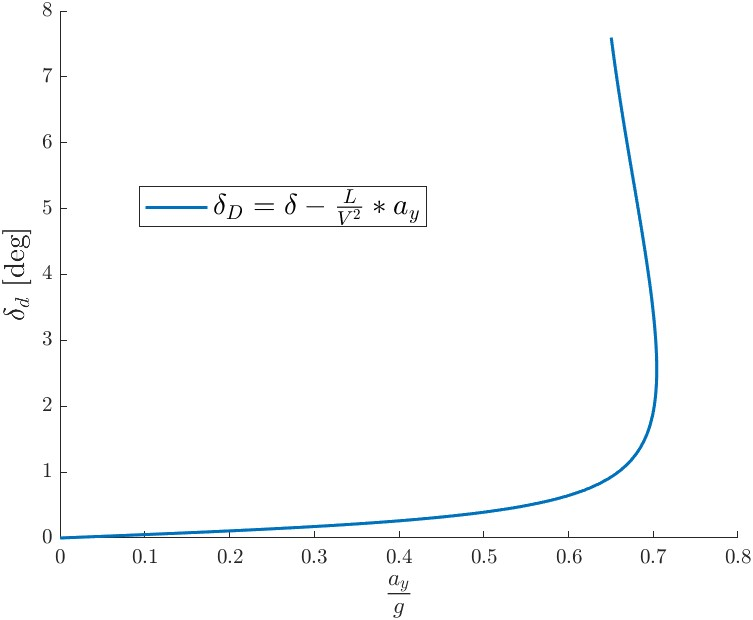
\includegraphics[scale=0.4]{Immagini/Understeer Gradient/Sterzo dinamico cinesi.jpg}
    \caption{}
    \label{fig:Sterzo Dinamico}
\end{figure}
$d\rho/da_y$ cambia il suo segno oltre il punto di flesso della curva:
Questo genera un ambiguità teorica per quanto riguarda la definizione di comportamento sovrasterzante o sottosterzante:\\
Nonostante sia chiaro il fatto che il veicolo nella pratica sia in completo scorrimento dell'assale anteriore
(completo sottosterzo), qualche ricercatore potrebbe esprimere dubbi sul fatto che oltre il punto di flesso riducendo
l'angolo di sterzo il veicolo riprenda direzionalità ($R$ diminuisce come nel caso di sovrasterzo).

\subsubsection{Critica di Guiggiani}
Il calcolo di $K$ necessita sia dell'angolo di sterzata $\delta_{ref}$ sia dell'angolo di sterzata di
Ackermann $\frac{l}{R}$.\\ 
Purtroppo, risultano ben definiti solo nel modello a singola traccia, mentre in un veicolo reale
risultano entrambi di ambigua definizione: le due ruote anteriori hanno tipicamente
angoli di sterzata differenti rendendo incerto l'angolo di sterzata $\delta_{ref}$.
Anche l'angolo di sterzata cinematica $\frac{l}{R}$ diventa ambiguo quando un veicolo è dotato
di tre o più assi, poiché il passo $l$ non è più definito chiaramente. Nonostante la maggior parte
delle auto dispongano di soli due assi, l'autore ritiene errato basare una teoria su un concetto
così debole.\\


%-----------------------------------------------------------------------------------------------------------
\section{Formulazioni alternative del gradiente di sottosterzo}
\subsubsection{Una nuova formulazione del gradiente di sottosterzo basata sulla velocità}
In questo sotto paragrafo si vuole descrivere ed analizzare una nuova formulazione proposta in un 
articolo di ricerca in fase di revisione.
L'articolo in questione è stato creato dagli autori He Zhen, Guan Yihang ,Zhou Hongliang del "Harbin 
institute of technology, School of Astronautics" e da Miao Weiwei, Yu zhen del "Chassis Department
FAW Group corporation".
il titolo "A new formulation of the understeer gradient and stability
margin to analyze vehicle steady-state cornering behaviour".\\

In questo articolo si propone una nuova formulazione che non sia dipendente dall'accelerazione
laterale in modo da evitare di incorrere nei problemi osservati precedentemente.
Questa nuova formulazione si propone per essere utilizzata in condizioni critiche 
(saturazione dei pneumatici) ed è definita dalla derivata della curvatura rispetto alla velocità: 
$K = \frac{\partial \rho}{\partial u}$ o $K = \frac{d \rho} {du}$\\ 
Può essere espressa in funzione della velocità d'imbardata:
\begin{equation} \label{Kcinesi}
K = \frac{d \rho}{du} = \frac{d(ru)}{du} = \frac{dr}{du} - \frac{r}{u}
\end{equation}

\begin{figure}[!h]
    \centering
    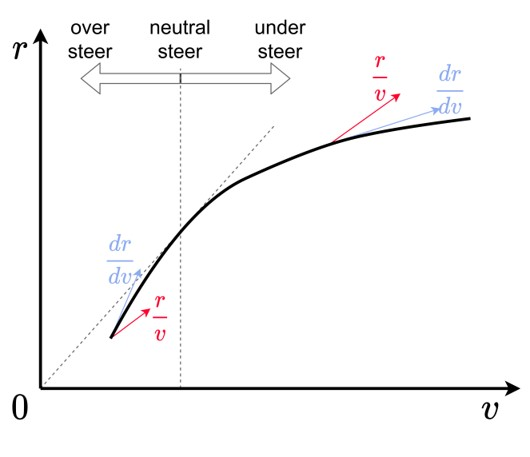
\includegraphics[scale=0.6]{Immagini/Understeer Gradient/K_cinesi.jpg}
    \caption{}
    \label{fig:K_cinesi}
\end{figure}
Il segno di $K$ è determinato dal numeratore, che è la differenza tra la pendenza tangente $\frac{dr}
{du}$ e la pendenza assoluta $\frac{r}{u}$ in ogni punto della curva $r$  $u$.\\ 
Questa differenza può essere ottenuta intuitivamente dalla curva stessa. La Fig.\ref{fig:K_cinesi} 
mostra che:\\ 
-Quando $\frac{dr}{du} > \frac{r}{u}$ e $K > 0$, la curvatura aumenta, indicando sovrasterzo.\\ 
-Quando $\frac{dr}{du} < \frac{r}{u}$ e $K < 0$, la curvatura diminuisce, indicando sottosterzo.\\
\'E sostanzialmente funzione di $r$ e $u$ e non coinvolge concetti complessi, questo la rende 
applicabile a diversi tipi di veicoli, come: veicoli a sterzata anteriore (tradizionale), veicoli a
quattro ruote sterzanti, veicoli a quattro ruote indipendenti e persino veicoli con più di quattro
ruote.\\ 
\'E applicabile a prove di "rampspeed" cioè con angolo di sterzo fissato e velocità crescente mentre
non è applicabile a prove di "rampsteer".
Questo rappresenta un difetto di questa nuova formulazione.\\
Inoltre eliminando la dipendenza dall'accelerazione laterale si perde il nesso con la stabilità del
veicolo del quale abbiamo parlato nel cap.\ref{cha:cap1}, per risolvere questo inconveniente gli
autori propongono l'aggiunta di un margine di stabilità, tuttavia rappresenta pur sempre un limite
di questa formulazione.


\subsubsection{Bucchi e Frendo}

Le formulazioni classiche concentrano l'attenzione sul controllo dell'imbardata del veicolo utilizzando modelli fortemente
semplificati sia per i pneumatici che per la dinamica del veicolo.\\
La nuova formulazione proposta nell'articolo \cite{doi:10.1080/00423114.2016.1167225} mette in relazione  il gradiente di
sottosterzo alla coppia d'imbardata, a partire da manovre quasi stazionarie facilmente eseguibili su veicoli reali.\\
Questa formulazione si basa sulla conoscenza della derivata (rispetto al tempo) della curvatura e del momento d'imbardata
generato dalle forze dei pneumatici.\\
\begin{figure}[!h]
    \centering
    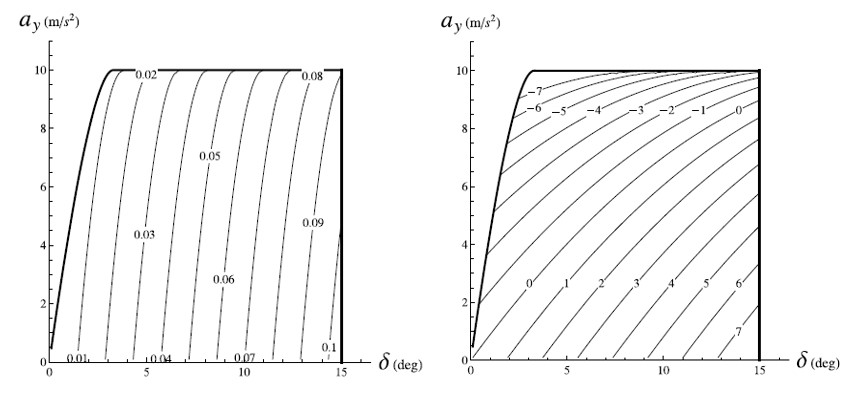
\includegraphics[scale=0.8]{Immagini/Understeer Gradient/Steadystate maps.jpg}
    \caption{Steadystate maps da \cite{guiggiani2018science}}
    \label{fig:Steadystate maps}
\end{figure}
Le mappe in figura \ref{fig:Steadystate maps} sono chiamate "steadystate maps", Le linee numerate
della mappa a sinistra rappresentano la curvatura mentre quelle a destra rappresentano l'angolo di
assetto $\beta$.\\
Creare le mappe per tutte le combinazioni di $\Tilde{a_y}$ e $\delta_W$ risulta dispendioso, per
questo motivo gli autori hanno deciso di considerare manovre a velocità costante ($\dot{u} = 0$) e 
($\dot{\delta_W} =$ costante) con lo scopo di ottenere informazioni sul comportamento dinamico del
veicolo considerato. Queste manovre possono essere considerate rappresentative (con buon
a approssimazione ) delle comuni azioni di guida.\\
A partire dalla mappa $\rho_p(\Tilde{a_y}, \delta_W)$, si può scrivere il differenziale:
\begin{equation}
   d\rho_p = \frac{\partial \rho_p}{\partial \Tilde{a_y}} d\Tilde{a_y} + \frac{\partial \rho_p}{\partial \delta_W} d\delta_W 
\end{equation}
Se $\delta_W(t)$ varia lentamente e $u = \text{costante}$ allora: \quad $\rho \approx \rho_p$ \quad e \quad  $a_y = 
\dot{\beta}u + \rho u^2 - \tilde{a}_y$.\\ 
In questo caso, le "steady-state map" ($\beta_p$ , $\rho_p$) possono comunque essere utilizzate per valutare la derivata
della curvatura $\dot{\rho}$ a partire dal differenziale $d\rho_p$ come segue:
\begin{equation} \label{17}
\dot{\rho} \cong \frac{\partial \rho}{\partial \tilde{a}_y} \dot{a}_y + \frac{\partial \rho}{\partial \delta_w} \dot{\delta}_w = - \frac{K}{l}\dot{a}_y + \frac{\tau}{l} \dot{\delta}_w
\end{equation}
Questa espressione non è generale e può essere considerata corretta solo nelle condizioni in cui la $\dot{\delta_W}$ sia relativamente bassa e $\beta$,$\rho$ possano essere approssimate dalle steady-state maps.\\
Il termine $\dot{a}_y$ può essere ottenuto a partire dalla definizione di accelerazione laterale per manovre a velocità costante:
\begin{equation} \label{18}
    \dot{a}_y = \frac{d(\dot{\beta}u + \rho u^2)}{dt} = \ddot{\beta}u + \dot{\rho}u^2 \cong \dot{\rho}u^2
\end{equation}
dove $\dot{u} = 0$   e  $\ddot{\beta}u \approx \dot{\rho}u^2$ (in condizioni di guida standard).\\ 
Sostituendo l'Eq. \ref{18} nell'Eq. \ref{17}, si ottiene una nuova definizione del gradiente di sottosterzo:
\begin{equation} \label{19}
    K \cong \frac{1}{u^2} \left( \frac{\tau \dot{\delta}_w }{\dot{\rho}} - l \right)    
\end{equation}
che può essere scritto in modo alternativo come una funzione del momento d'imbardata $N$:
\begin{equation} \label{20}
    K \cong \frac{1}{u^2} \left( \frac{\tau \dot{\delta}_wJu}{N} - l \right)
\end{equation}
%L'eq. \ref{19} consente di valutare il gradiente di sottosterzo sulla base di $\dot{\delta}_W$ e $\dot{\rho}$, misurabili attraverso un encoder sul volante e due accelerometri in due posizioni diverse del veicolo. \\
L'efficacia dell'eq.\ref{19}, deriva dal fatto che $K$ possa essere ricavato sperimentalmente eseguendo manovre quasi-
stazionarie a velocità costante, misurando facilmente $\dot{\delta}_W$ e $\dot{\rho}$ attraverso un encoder sul volante e 
due accelerometri in due posizioni diverse del veicolo. \\
Se la velocità del volante $\dot{\delta}_W$ viene mantenuta costante, il momento d'imbardata è inversamente correlato al
gradiente di sottosterzo (\ref{20}):\\ 
All'aumentare del momento d'imbardata, $K$ diminuisce $\xrightarrow{}$ il veicolo diventa più sovrasterzante.\\
Nel caso $N = 0$ possono verificarsi tre circostanze:\\ 
$\bullet$ Se $\dot{\delta}_W = 0$ l'eq. \ref{20} è indeterminata, tuttavia essendo in condizioni stazionarie possiamo
calcolare il gradiente di sottosterzo con la formulazione classica.\\
$\bullet$ Se $\dot{\delta}_W \neq 0$, $K$ tende all'infinito, significa che la curvatura non varia nonostante la velocità
di rotazione del volante sia diversa da zero.\\
In particolare,
se $\dot{\delta}_W > 0$ si verifica il sottosterzo poiché la velocità d'imbardata del veicolo non aumenta anche se il
conducente sta aumentando l'angolo di sterzo.\\ 
Al contrario, se $\dot{\delta}_W < 0$ si verifica il sovrasterzo poiché la velocità d'imbardata del veicolo rimane costante
anche se il conducente sta controsterzando.\\ 
attraverso lo sviluppo del torque vectoring, 
in quanto collega la definizione classica del sottosterzo al momento d'imbardata.

%--------------------------------------------------------------------------------------------------------------------
\section{Nuovo approccio all'handling}
Massimo Guiggiani sviluppò un nuovo approccio al comportamento direzionale degli autoveicoli per ovviare ad alcune
incertezze presentate nei paragrafi precedenti, quali:\\
$\bullet$ La difficoltà nel definire un veicolo cinematico di riferimento\\
$\bullet$ La difficoltà nella definizione del passo nei veicoli con più di due assi\\
$\bullet$ La mancanza di un chiaro legame tra il gradiente misurato in prove stazionarie e il comportamento del veicolo nei
transitori.\\
La soluzione proposta prevede un metodo che non faccia uso del veicolo cinematico di riferimento e del modello
monotraccia.\\
Si definisce globalmente un veicolo senza porre attenzione sui dettagli, non si fà riferimento al numero e alla
disposizione delle ruote ne tantomeno ai loro eventuali angoli di sterzo.
Le cui equazioni del moto possono essere scritte nella forma:
\begin{equation} \label{eq:Y e N 1}
  \begin{split}
     m(\dot{v} + ur) & = \Tilde{Y} (v,r;u,\delta_v) \\
     J \dot{r} & = \Tilde{N} (v,r;u,\delta_v)
  \end{split}
\end{equation}
Con riferimento alla curvatura $\rho$ e l'angolo di assetto $\beta$:
\begin{equation} \label{eq:Y e N}
  \begin{split}
     m(u\dot{\beta} + \dot{u}\beta + u^2\rho) & = Y (\beta,\rho;u,\delta_v)\\
     J (u\dot{\rho} + \dot{u} \rho) & = N (\beta,\rho;u,\delta_v)
  \end{split}
\end{equation}
Introduciamo le "derivate di stabilità", esse sono le derivate parziale delle equazioni \ref{eq:Y e N} rispetto a
$\beta$ e $\rho$:
  \begin{align}
     Y_{\beta}=\frac{\partial{Y}}{\partial{\beta}} \qquad \quad &  Y_{\rho}=\frac{\partial{Y}}{\partial{\rho}} & N_{\beta}=\frac{\partial{N}}{\partial{\beta}} \qquad \quad &  N_{\rho}=\frac{\partial{N}}{\partial{\rho}}
  \end{align}
\subsubsection{Applicazione al modello monotraccia lineare}
A titolo di esempio si mostra l'applicazione al modello monotraccia lineare in \cite{guiggiani2007dinamica}.
Definiamo $\delta_1$ e $\delta_2$ rispettivamente l'angolo di sterzo anteriore e posteriore:\\
\begin{align}
     \delta_1 = \tau_1 \delta_v \qquad & \qquad \delta_2 = \tau_2 \delta_v = \tau_1 \chi \delta_v
\end{align}
L'eq.\ref{eq:Y e N 1} nel caso del modello monotraccia lineare diventano:
\begin{equation} \label{eq:equazioni del moto guiggiani}
  \begin{split}
     m(\dot{v} + ur) & = -(\frac{C_1 + C_2}{u})v - (\frac{C_1a_1-C_2a_2}{u})r + (C_1+\chi C_2)\tau_1 \delta_v \\
     J \dot{r} & = -(\frac{C_1a_1-C_2a_2}{u})v - (\frac{C_1a_1^2+C_2a_2^2}{u})r + (C_1a_1-\chi C_2a_2)\tau_1 \delta_v \\
  \end{split}
\end{equation}
Le derivate di stabilità saranno dunque:
\begin{align}
     Y_{\beta} & =-(C_1+C_2) \qquad \quad &  N_{\beta} & =-(C_1a_1-C_2a_2) \\
     Y_{\rho} & = -(C_1a_1-C_2a_2) \qquad \quad &  N_{\rho} & = -(C_1a_1^2+C_2a_2^2)\\
     Y_{\delta} & =(C_1+\chi C_2)\tau_1 \qquad \quad &  N_{\delta} & =(C_1a_1-\chi C_2a_2)\tau_1
\end{align}
Le ultime due rappresentano le derivate parziali rispetto a $\delta$:
  \begin{align}
     Y_{\delta}=\frac{\partial{Y}}{\partial{\delta}} \qquad \quad &  N_{\delta}=\frac{\partial{N}}{\partial{\delta}}
  \end{align}
Le equazioni del moto \ref{eq:equazioni del moto guiggiani} in condizioni di equilibrio possono essere riscritte in 
funzione di $\beta$ e $\rho$, introducendo $\Tilde{a_y}$ (accelerazione laterale a regime).\\
\begin{equation} \label{eq:equazioni del moto regime}
  \begin{split}
     m\Tilde{a_y} & = -(C_1+C_2)\beta_p - (C_1a_1-C_2a_2)\rho_p + (C_1+\chi C_2)\tau_1 \delta_v \\
     0 & = -(C_1a_1-C_2a_2)\beta_p - (C_1a_1^2+C_2a_2^2)\rho_p + (C_1a_1-\chi C_2a_2)\tau_1 \delta_v \\
  \end{split}
\end{equation}
Per definizione, \(\dot{v} = \dot{r} = 0\), cioè \(\beta = \rho = 0\).\\ 
Il conducente ha controllo diretto su \(u\) e \(\delta v\), che vengono mantenuti costanti.\\
Il pedice \(a\) rappresenta i "valori di assetto".\\
L'equazioni del moto possono essere risolte per ottenere le "steady-state maps":\\
\begin{equation} 
  \begin{split}
     \beta_p = \hat{\beta}_p(u_a, \delta_{va}) = \frac{v_p(u_a, \delta_{va})} {u_a} \\
     \rho_p = \hat{\rho}_p(u_a, \delta_{va}) = \frac{r_p(u_a, \delta_{va})} {u_a}
  \end{split}
\end{equation}
Applicando questo metodo al comportamento transitorio conviene sostituire $u_a = u_a(\delta v_a, \tilde{a}_y)$:
\begin{equation} 
  \begin{split}
     \beta_p = \beta_p(\delta_{va}, \tilde{a}_y) = \hat{\beta}_p(u_a(\delta_{va}, \tilde{a}_y), \delta_{va}) \\
     \rho_p = \rho_p(\delta_{va}, \tilde{a}_y) = \hat{\rho}_p(u_a(\delta_{va}, \tilde{a}_y), \delta_{va})
  \end{split}
\end{equation}
\begin{equation} \label{eq:5.75}
  \begin{split}
     \beta_p = \beta_p(\delta_{va}, \tilde{a}_y) = \frac{v_p}{u_a} = (\frac{a_2 a_1\chi}{l})\tau_1 \delta_{va} - \frac{m}{l^2} (\frac{C_1a_1^2+C_2a_2^2}{C_1C_2})\tilde{a}_y\\
     \rho_p = \rho_p(\delta_{va}, \tilde{a}_y) = \frac{r_p}{u_a} = (\frac{1-\chi}{l})\tau_1 \delta_{va} - \frac{m}{l^2} (\frac{C_2a_2-C_1a_1}{C_1C_2})\tilde{a}_y\\
  \end{split}
\end{equation}
Derivando le equazioni \ref{eq:5.75} rispetto ad $\tilde{a}_y$ e $\delta_{va}$:
\begin{align}
     \beta_y & =- \frac{m}{l^2} (\frac{C_1a_1^2+C_2a_2^2}{C_1C_2}) \qquad \quad &  \beta_{\delta} & =(\frac{a_2 +\chi a_1}{l})\tau_1 \\
     \rho_y & = - \frac{m}{l^2} (\frac{C_2a_2-C_1a_1}{C_1C_2}) \qquad \quad &  \rho_{\delta} & = (\frac{1-\chi}{l})\tau_1
\end{align}
Si tratta di quantità ottenibili per via sperimentale eseguendo manovre stazionarie, a titoli di esempio sono state 
ricavate analiticamente nel caso del modello monotraccia lineare,
  \begin{align*}
     s_1 & =\beta_y = - \frac{m}{l^2} (\frac{C_2a_2^2+C_1a_1^2}{C_1C_2}) & = & - \frac{m}{(a_1+a_2)^2} (\frac{\Phi_2a_2^2+\Phi_1a_1^2}{\Phi_1\Phi_2})\\
     s_2 & =\rho_y = - \frac{m}{l^2} (\frac{C_2a_2-C_1a_1}{C_1C_2}) & = & - \frac{m}{(a_1+a_2)^2} (\frac{\Phi_2a_2-\Phi_1a_1}{\Phi_1\Phi_2})\\
     s_3 & =\beta_{\delta}= \tau_1 \frac{a_2+\chi a_1}{l} & = & \tau \frac{(1+k)a_2+k a_1}{a_1+a_2}\\
     s_4 & =\rho_{\delta}= \tau_1 \frac{1-\chi}{l} & = & \tau \frac{(1+k)-k}{a_1+a_2} = \frac{\tau}{a_1+a_2}\\
     s_5 & =\frac{N_{\delta}}{J}= \tau_1 \frac{C_1a_1-\chi C_2a_2}{J} & = & \tau \frac{(1+k)\Phi_1a_1-k \Phi_2a_2}{J}\\
     s_6 & =\frac{Y_{\delta}}{J}= \tau_1 \frac{C_1 + \chi C_2}{m} & = & \tau \frac{(1+k)\Phi_1 + k \Phi_2}{m}\\
  \end{align*}
Per chiarezza della trattazione sono state riportate due versioni che si trovano in letteratura, equivalenti tra loro con
piccole differenze nella simbologia.
Questi sei handling bricks dipendono da sette parametri di progettazione, 
Dunque possono esistere infiniti veicoli diversi che condividono gli stessi valori degli $s_i$.

\subsubsection{Veicoli differenti con comportamento analogo}
In questo paragrafo si mostreranno delle prove nel quale si mostra l'attendibilità di questo nuovo approccio.\\
"Veicoli diversi avranno lo stesso comportamento direzionale solo se hanno gli stessi valori di tutti e sei gli handling
bricks".\\
Per avere una visione chiara di quest'idea, nell'ambito di questa tesi sono state replicate le prove a pag.325-327 di \cite{guiggiani2018science}.\\
La prova consiste in un colpo di sterzo $\delta_v$ partendo da una velocità in rettilineo di 30 [m/s].\\
\begin{table}[htbp]
  \centering
  \footnotesize
  \begin{tabular}{@{}|c|c|c|c|c|c|c|c|c|c|@{}}
    \hline
    $k$   & $\Phi_1$    & $\Phi_2$    & $a_1$   & $a_2$   & $J_z$   & $m$    & $\tau$    & $K$    & $-\rho_y$ \\
     & [N/rad] & [N/rad] & [m] & [m] & [kg m^2] & [kg] &  & [deg/g] & [deg/(mg)] \\
    \hline
    -0.10 & 86332 & 73668 & 0.73 & 1.86 & 2000 & 1300 & 0.99/20 & 3.28 & 1.27 \\
    \hline
    0.00  & 70000 & 90000 & 1.00 & 1.60 & 2000 & 1300 & 1.00/20 & 3.30 & 1.27 \\
    \hline
    +0.10 & 49065 & 110935& 1.48 & 1.32 & 2000 & 1300 & 1.08/20 & 3.55 & 1.27 \\
    \hline
  \end{tabular}
  \caption{Parametri costruttivi di 3 veicoli differenti ma con comportamento analogo in transitorio}
  \label{tab:table 7.1}
\end{table}

\begin{figure}[!h]
    \centering
    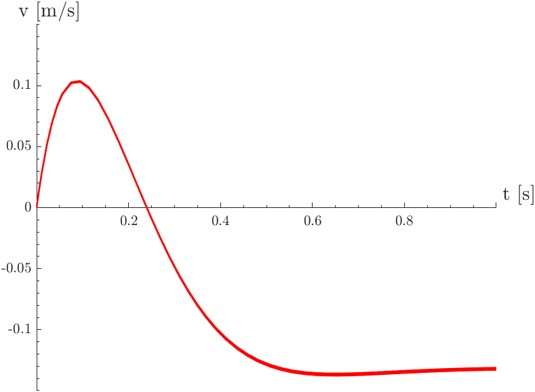
\includegraphics[scale=0.6]{Immagini/Understeer Gradient/table7.1 v.jpg}
    \caption{velocità laterale dei tre veicoli tab.\ref{tab:table 7.1}}
    \label{fig:table7.1 v}
\end{figure}

\begin{figure}[!h]
    \centering
    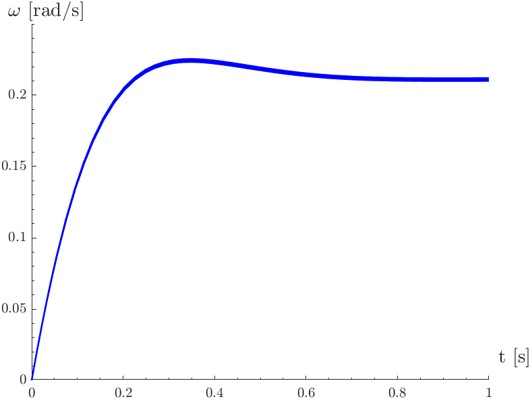
\includegraphics[scale=0.6]{Immagini/Understeer Gradient/table7.1 r.jpg}
    \caption{velocità d'imbardata dei tre veicoli tab.\ref{tab:table 7.1}}
    \label{fig:table7.1 r}
\end{figure}

\begin{figure}[!h]
    \centering
    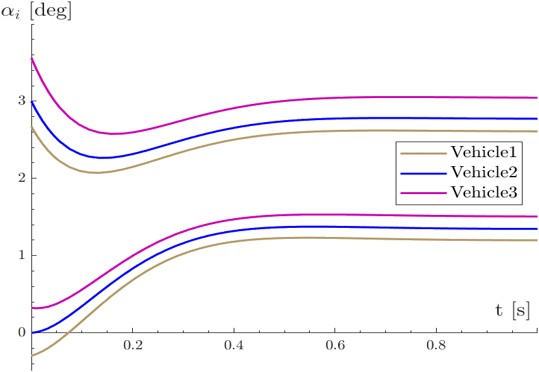
\includegraphics[scale=0.6]{Immagini/Understeer Gradient/table7.1 alfa.jpg}
    \caption{angoli di deriva dei tre veicoli tab.\ref{tab:table 7.1}}
    \label{fig:table7.1 alfa}
\end{figure}

\begin{table}[htbp]
  \centering
  \footnotesize
  \begin{tabular}{@{}|c|c|c|c|c|c|c|c|c|c|@{}}
    \hline
    $k$   & $\Phi_1$    & $\Phi_2$    & $a_1$   & $a_2$   & $J_z$   & $m$    & $\tau$    & $K$    & $-\rho_y$ \\
    $[-]$ & $[N/rad]$ & $[N/rad]$ & $[m]$ & $[m]$ & $[kg m^2]$ & $[kg]$ & $[-]$ & $[deg/g]$ & $[deg/(mg)]$ \\
    \hline
    -0.60 & 141316 & 18684 & 0.01 & 4.01 & 2000 & 1300 & 1.55/20 & 5.10 & 1.27 \\
    \hline
    0.00  & 70000 & 90000 & 1.00 & 1.60 & 2000 & 1300 & 1.00/20 & 3.30 & 1.27 \\
    \hline
     +0.166& 22426  & 137574& 2.73 & 0.98 & 2000 & 1300 & 1.42/20 & 4.71 & 1.27 \\
    \hline
  \end{tabular}
  \caption{Parametri costruttivi di 3 veicoli differenti con angolo di sterzo posteriore k elevato}
  \label{tab:table 7.2}
\end{table}

\begin{figure}[!h]
    \centering
    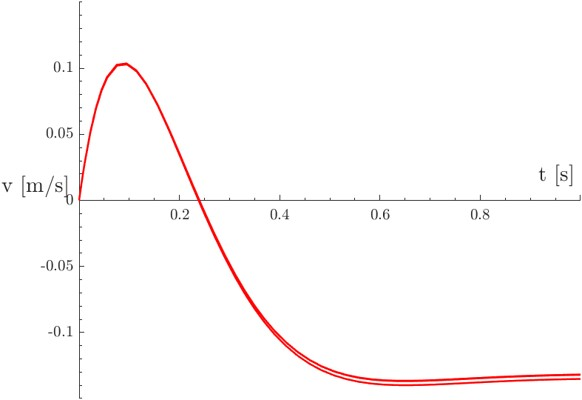
\includegraphics[scale=0.6]{Immagini/Understeer Gradient/table7.2.jpg}
    \caption{velocità laterale dei tre veicoli tab.\ref{tab:table 7.2}}
    \label{fig:table7.2 v}
\end{figure}

\begin{figure}[!h]
    \centering
    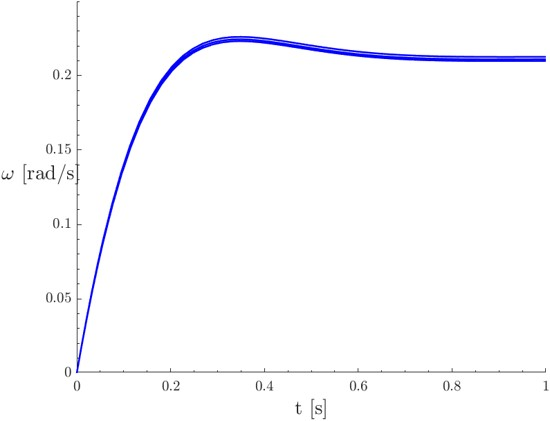
\includegraphics[scale=0.6]{Immagini/Understeer Gradient/table7.2 r.jpg}
    \caption{velocità d'imbardata dei tre veicoli tab.\ref{tab:table 7.2}}
    \label{fig:table7.2 r}
\end{figure}
Per contro prova si è verificato come possano esistere veicoli che pur condividendo lo stesso $K$ e lo stesso $\rho_y$ 
presentino un comportamento direzionale differente, questo permette di mostrare la parzialità del $K$ e sottolineare
l'importanza di avere una visione completa su tutti e sei le derivate.\\
Fissato il valore di $\rho_y$ si è variata la Cornering stiffness dell'assale anteriore e ricavata quella dell'assale
posteriore, mantenendo costanti gli altri parametri.\\

\begin{table}[htbp]
  \centering
  \footnotesize
  \begin{tabular}{@{}|c|c|c|c|c|c|c|c|c|c|@{}}
    \hline
    $k$   & $\Phi_1$    & $\Phi_2$    & $a_1$   & $a_2$   & $J_z$   & $m$    & $\tau$    & $K$    & $-\rho_y$ \\
    $[-]$ & $[N/rad]$ & $[N/rad]$ & $[m]$ & $[m]$ & $[kg m^2]$ & $[kg]$ & $[-]$ & $[deg/g]$ & $[deg/(mg)]$ \\
    \hline
    0.00  & 70000 & 90000 & 1.00 & 1.60 & 2000 & 1300 & 1.00/20 & 3.30 & 1.27 \\
    \hline
    0.00  & 65000 & 77724.45 & 1.00 & 1.60 & 2000 & 1300 & 1.00/20 & 3.30 & 1.27 \\
    \hline
    0.00  & 75000 & 104341.51 & 1.00 & 1.60 & 2000 & 1300 & 1.00/20 & 3.30 & 1.27 \\
    \hline
    0.00  & 72000 & 95485.43 & 1.00 & 1.60 & 2000 & 1300 & 1.00/20 & 3.30 & 1.27 \\
    \hline
    0.00  & 60000 & 67036.50 & 1.00 & 1.60 & 2000 & 1300 & 1.00/20 & 3.30 & 1.27 \\
    \hline
    0.00  & 80000 & 121203.60 & 1.00 & 1.60 & 2000 & 1300 & 1.00/20 & 3.30 & 1.27 \\
    \hline
    0.00  & 56000 & 59445.93 & 1.00 & 1.60 & 2000 & 1300 & 1.00/20 & 3.30 & 1.27 \\
    \hline
    0.00  & 84000 & 137020.11 & 1.00 & 1.60 & 2000 & 1300 & 1.00/20 & 3.30 & 1.27 \\
    \hline
  \end{tabular}
  \caption{Parametri costruttivi di differenti veicoli che condividono lo stesso $\rho_y$}
  \label{tab:table 7.3}
\end{table}
\begin{table}[htbp]
  \centering
  \begin{tabular}{@{}|c|c|c|c|c|c|@{}}
    \hline
     $s_1$   & $s_2$   & $s_3$   & $s_4$   & $s_5$   & $s_6$\\
     \hline
    -5.16 & -1.27 & 0.03 & 0.02 & 1.75 & 2.69 \\
    \hline
    -5.65 & -1.27 & 0.03 & 0.02 & 1.63 & 2.50 \\
    \hline
    -4.73 & -1.27 & 0.03 & 0.02 & 1.88 & 2.88 \\
    \hline
    -4.98 & -1.27 & 0.03 & 0.02 & 1.80 & 2.77 \\
    \hline
    -6.23 & -1.27 & 0.03 & 0.02 & 1.50 & 2.31 \\
    \hline
    -4.35 & -1.27 & 0.03 & 0.02 & 2.00 & 3.08 \\
    \hline
    -6.76 & -1.27 & 0.03 & 0.02 & 1.40 & 2.15 \\
    \hline
    -4.09 & -1.27 & 0.03 & 0.02 & 2.10 & 3.23 \\ 
    \hline
  \end{tabular}
  \caption{Rispettivi handling bricks dei veicoli in tab.\ref{tab:table 7.3}}
  \label{tab:table 7.3 s}
\end{table}

\begin{figure}[!h]
    \centering
    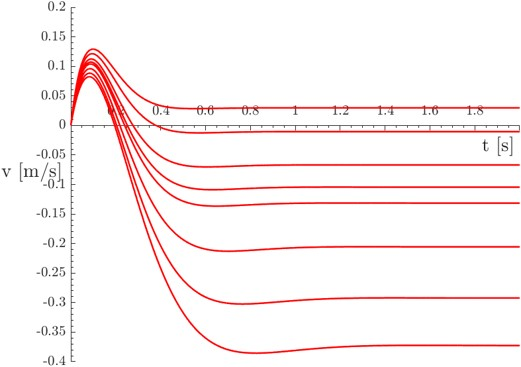
\includegraphics[scale=0.6]{Immagini/Understeer Gradient/table manuel v.jpg}
    \caption{velocità laterale veicoli tab.\ref{tab:table 7.3}}
    \label{fig:table7.3 v}
\end{figure}

\begin{figure}[!h]
    \centering
    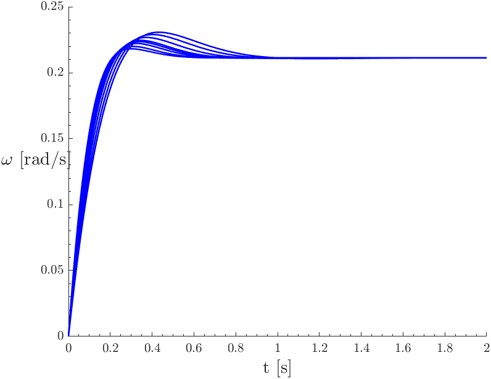
\includegraphics[scale=0.6]{Immagini/Understeer Gradient/table manuel r.jpg}
    \caption{velocità d'imbardata veicoli tab.\ref{tab:table 7.3}}
    \label{fig:table7.3 r}
\end{figure}
Le fig.\ref{fig:table7.3 v} e \ref{fig:table7.3 r} mostrano come i veicoli pur avendo lo stesso valore di $K$ mostrino
comportamenti abbastanza differenti.

%----------------------------------------------------------------------------------------------------------------
\section{Metodi per la misura del sottosterzo}
\subsection{ISO-4138-2021}
La normativa ISO 4138 specifica metodi di test "open loop" per determinare il comportamento direzionale di autovetture stradali (ISO 3833) e di camion leggeri.\\
Il comportamento direzionale riguarda la dinamica del veicolo in generale e la "tenuta di strada"
Le manovre "open loop" descritte in seguito non sono rappresentative delle condizioni reali di guida, ma sono comunque molto utili per ottenere misure del comportamento complessivo del veicolo a seguito di diversi tipi di input di controllo e sotto condizioni di prova rigidamente definite.
I tre metodi definiti dalla normativa \cite{iso4138} sono:
\begin{enumerate}
    \item "Costant-speed test method"
    \item "Costant-steering-wheel angle test method"
    \item "Costant-radius test method"
\end{enumerate}
\subsubsection{Costant-speed test method}
Questo metodo di prova prevede che il veicolo sia condotto con velocità velocità costante variando l'angolo di sterzo.\\
Le caratteristiche direzionali sono determinate dai dati ricavati rispetto all'accelerazione laterale ma potrebbe
richiedere ampie aree di test, a seconda della combinazione di velocità e accelerazione laterale. \\
La variazione dell'angolo di sterzo dovrebbe essere più accurata possibile per garantire affidabilità dei dati.\\
La velocità di riferimento della prova è 100 [km/h], ma possono essere eseguite prova a diverse velocità.\\
Viene comunemente chiamato "rampsteer" (rampa di sterzo).\\
\subsubsection{Costant-steering-wheel angle test method}
Questo metodo di prova prevede che il veicolo sia condotto con velocità velocità crescente ed un angolo di sterzo mantenuto fisso.\\ 
Il raggio percorso sarà funzione della velocità di avanzamento e dell'accelerazione laterale.\\
Il test può essere eseguito con una serie di prove discrete oppure con una singola prova continua.\\
Nella prima, l'angolo dello sterzo viene applicato con il veicolo che viaggia a velocità discrete e viene mantenuto fino a quando non si raggiungono condizioni stazionarie.\\ 
Nella seconda, l'angolo dello sterzo viene mantenuto fisso mentre la velocità aumenta in modo lento e continuo fino al limite di controllo.\\
L'angolo di sterzo dovrà fornire un raggio percorso a bassa velocità di almeno 30 [m] e minimo 20 [m] valore limite.\\
Viene comunemente chiamato "rampspeed" (rampa di velocità).
\subsubsection{Costant-radius test method}
Questo metodo di prova prevede che il veicolo sia condotto a diverse velocità su un percorso circolare di raggio definito. Il raggio di curvatura di riferimento è solitamente 100 [m], possono essere utilizzati raggi maggiori e minori, Viene raccomandato un valore minimo di 40 [m]. \\
Le caratteristiche di risposta direzionale sono determinate attraverso i dati ottenuti.\\
Questa procedura può essere condotta in un'area relativamente piccola risultando adatta alle strutture esistenti nel quale
possa essere individuata una circonferenza sufficientemente ampia, può essere svolta in due varianti: \\
-Nella prima il veicolo percorre un percorso circolare a velocità discrete e costanti. 
I dati vengono rilevati quando viene raggiunto lo stato stazionario. 
Il test può essere eseguito su qualsiasi percorso livellato a raggio costante di lunghezza sufficiente per raggiungere e 
mantenere lo stato stazionario a raggio costante per almeno un periodo di misurazione di 3 s.\\
-Nella seconda, il veicolo rimane sul cerchio con un continuo e lento aumento di velocità, durante il quale vengono
rilevati i dati. La derivata dell'accelerazione laterale dovrebbe essere di 0,1 [m/s²/s] con un limite massimo di [0,2 m/s²/s].


